\documentclass[../../main.tex]{subfiles}

\begin{document}

\section{Medición de capacitores}

\begin{figure}[H]	
	\centering
	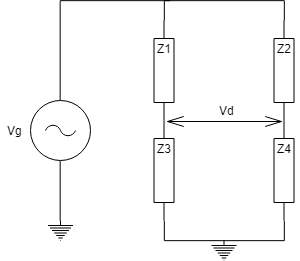
\includegraphics[width=0.35\textwidth]{fotos/PuenteGen.png}
	\caption{Puente con Impedancias genericas} \label{fig:pgc}
\end{figure}

Se diseñó un puente que permita medir capacitores, en un rango de capacidad $C \in [10nF,100nF]$ y en un rango de factor de disipación $D \in[0.015 , 0.09 ] $, para una frecuencia de 10KHz. 
\par Partiendo del puente de la figura \ref{fig:pgc}, donde $V_d=\frac{Z_3}{Z_1+Z_3} -\frac{Z_4}{Z_4 + Z_2}$, en el equilibrio $Z_1 Z_4 = Z_2  Z_3$.  Reemplazando $Z_1= R_1 + \frac{1}{SC_1}$, $Z_2= R_x + \frac{1}{SC_x}$, $Z_3=R_3$ y $Z_4=R_4$. En el equilibrio se cumple que $C_x=\frac{C_1 R_3}{R_4}$, $R_x=\frac{R_1 R_4}{R_3}$ y $D_x=2 \pi f C_1 R_1$.

\subsection{Elección de componentes}
Fijando $C_1=3nF$ y $R_3=1K \Omega$, y a partir de las ecuaciones  $C_x=\frac{C_1 R_3}{R_4}$ y $D_x=2 \pi f C_1 R_1$, se obtuvieron los valores de las variables de ajuste, $R_1 \in \left[  \frac{D_{min}}{2 \pi f C_1 R_1} ,  \frac{D_{max}}{2 \pi f C_1 R_1}  \right] = \left[ 79.5\Omega , 477.46 \Omega   \right]$ y 
$R_4 \in \left[ \frac{C_1 R_3}{C_{Xmax}} , \frac{C_1 R_3}{C_{Xmin}} \right]=   \left[ 30\Omega , 300 \Omega   \right]$.
\par La resitencia $R_1$ se implementó con una resistencia de $68 \Omega$ en serie con dos presets de $200 \Omega$ y la resistencia $R_4$ se implementó con una resistencia de $20\Omega$ en seire con un preset de $200 \Omega$ y otro de $100 \Omega$.

\subsection{Analisis de sensivilidades}
Para analizar la sencivilidad del puente, se grafico el cosciente de la sencivilidad de $V_d$ respecto de $R_1$ y $R_2$. y el objetivo es que dicho cociente se encuentre lo mejor posible ditribuido entre 0 y 1.
Con los valores de los componentes indicados anterioremente se obtuvo el siguiente grafico del cosiente de las sencivilidades
\begin{figure}[H]	
	\centering
	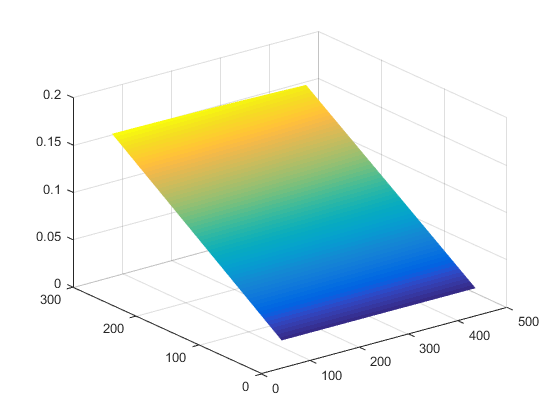
\includegraphics[width=0.7\textwidth]{fotos/sen.png}
	\caption{Cosciente de sencivilidades} 
\end{figure}
Como se observa en el grafico al variar $R_1$ y $R_4$ se obtuvo una superficie acotada entre 0 y 1.

\subsection{Calculo del error}
Para calcular el error en la maedicion se tuvo que distinguir cuales fueron las fuentes de error en la medicion, supusimos que el error en analizador de impedancias es despreciable.
Las fuentes de error que supusimos fueron las siguientes:
\begin{itemize}  
\item El error en la medición de las resistencias por parte del ohmetro lo cosnideramos de $1\Omega$
\item Como $V_d$ nunca llega a cero, y como la medicon se realizo con el voltimetro de banco consideramos que el error en la medicion de $V_d$ es de 1mv \ldots 
\end{itemize}

Conociendo que constructivamente $R_1$ y $R_4$ se realizaron con presets de $200\Omega$, estiamos el$\Delta R_1=\Delta R_2=2\Omega$ (un cuarto de vuelta del preset).

$$S_{R_1}^{V_d} \Delta R_1=\Delta V_d$$
$$\Delta R_1 = 8\Omega$$

Considerando el peor caso cuando se suman los errores, para $\Delta R_1 = 8\Omega$, ahora calculamos para $C_x$.
$$\Delta C_x = C_1 R_3 \frac{\Delta R_4}{R_4^2} $$
como en el peor caso $R_4=30\Omega$
$$\Delta C_x=3nF $$
y por ultimo, hay que hallar el error en $D_x$. Como $D_x=2\pi f  C_1 R_1$, entonces:
$$ \Delta D_x= 2 \pi  f  C_1 \cdot \Delta R_1 $$
$$ \Delta D_x=0.0009$$

\subsection{Convergencia}
Se analizo si el puente convergia para un unico valor de $R_1$ a un unico $D_x$ y $R_4$ a un unico $C_x$. Para ello se grafico vd en funcion de $C_x$ y $R_4$ en un caso y $R_1$ , $D_x$ para el otro.

\begin{figure}[H]	
	\centering
	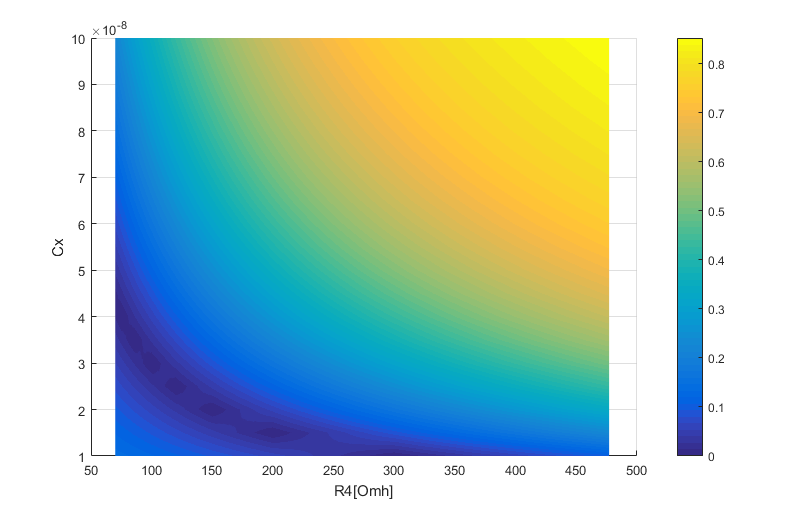
\includegraphics[width=0.7\textwidth]{fotos/conv_cx.png}
	\caption{Convergencia de $V_d$ respecto de $R_4$ y $C_x$ } 
\end{figure}

\begin{figure}[H]	
	\centering
	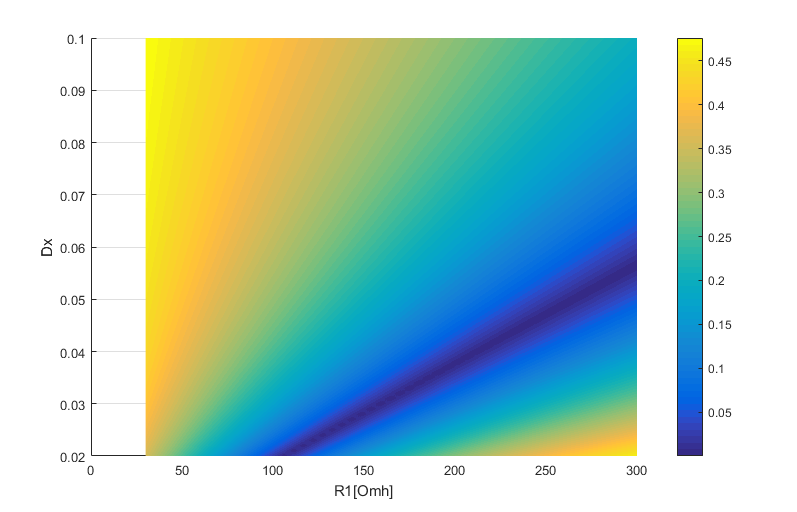
\includegraphics[width=0.7\textwidth]{fotos/conv_dx.png}
	\caption{Convergencia de $V_d$ respecto de $R_1$ y $D_x$ } 
\end{figure}

Como se observa en ambas figuras hay una unica franja violeta (minimo) de $V_d$, por ende la convergancia del puente es unica para cada $C_x$ y $D_x$.

\subsection{Manual de uso}
Para poder medir en el puente, se recomienda primero ajustar el preset correspoendiente a $R_4$, devido a que la sencivilidad del puentes es mallor respecto a dicha reisitencia, encontrando el minimo de $V_d$. Despues variar $R_1$ para minimizar aun mas $V_d$. Posteriormente desconectar todos los elementos del puente y medir las resistencias $R_4$ y $R_1$. Finalmente con las ecuaciones anteriormente mencionadas se obtiene el valor del capacitor medido, donde $C_x=\frac{C_1 R_3}{R_4}$, $R_x=\frac{R_1 R_4}{R_3}$ y $D_x=2 \pi f C_1 R_1$.

\subsection{Mediciones}
Se midieron los capacitores con el analizador de impedancias y con el puente.

\subsubsection{Analizador de impedancia}

\begin{table}[H]
\begin{center}
\begin{tabular}{|l|l|l|}
\hline
 Frecuencia&C&D\\
\hline \hline

$ 1KHz$ &9.8nf&0.015  \\ \hline
$ 10KHz$  & 9.6nF&0.023  \\ \hline
$ 100KHz$  &9.3nF &0.085  \\ \hline

\end{tabular}
\caption{Capacitor minimo } 
\end{center}
\end{table}
\begin{table}[H]
\begin{center}
\begin{tabular}{|l|l|l|}
\hline
 Frecuencia&C&D\\
\hline \hline

$ 1KHz$ &47.24nf&0.019  \\ \hline
$ 10KHz$  & 26nF&0.003 \\ \hline
$ 100KHz$  &43.56nF &0.08  \\ \hline

\end{tabular}
\caption{Capacitor medio } 
\end{center}
\end{table}

\begin{table}[H]
\begin{center}
\begin{tabular}{|l|l|l|}
\hline
 Frecuencia&C&D\\
\hline \hline

$ 1KHz$ &108nf&0.018  \\ \hline
$ 10KHz$  & 108nF&0.024  \\ \hline
$ 100KHz$  &102nF &0.083  \\ \hline

\end{tabular}
\caption{Capacitor maximo } 
\end{center}
\end{table}

\begin{table}[H]
\begin{center}
\begin{tabular}{|l|l|l|}
\hline
 Frecuencia&C&D\\
\hline \hline

$ 1KHz$ &186nf&0.01  \\ \hline
$ 10KHz$  & 181nF&0.016  \\ \hline
$ 100KHz$  &171nF &0.08  \\ \hline

\end{tabular}
\caption{Capacitor doble del maximo } 
\end{center}
\end{table}



\subsubsection{Puente}
Se midió $V_d$ con el voltimetro de banco

\begin{table}[H]
\begin{center}
\begin{tabular}{|l|l|l|}
\hline
 Frecuencia&C&D\\
\hline \hline

$ 1KHz$ &9.87nf&0.005  \\ \hline
$ 10KHz$  & 9.9nF&0.013  \\ \hline
$ 100KHz$  &9.58nF &0.1  \\ \hline

\end{tabular}
\caption{Capacitor minimo } 
\end{center}
\end{table}
\begin{table}[H]
\begin{center}
\begin{tabular}{|l|l|l|}
\hline
 Frecuencia&C&D\\
\hline \hline

$ 1KHz$ &44.8nf&0.0013  \\ \hline
$ 10KHz$  & 45.5nF&0.012 \\ \hline
$ 100KHz$  &42.4nF &0.13  \\ \hline

\end{tabular}
\caption{Capacitor medio } 
\end{center}
\end{table}

\begin{table}[H]
\begin{center}
\begin{tabular}{|l|l|l|}
\hline
 Frecuencia&C&D\\
\hline \hline

$ 1KHz$ &108nf&0.0013  \\ \hline
$ 10KHz$  & 108nF&0.013  \\ \hline
$ 100KHz$  &89.6nF & 0.14 \\ \hline

\end{tabular}
\caption{Capacitor maximo } 
\end{center}
\end{table}

\begin{table}[H]
\begin{center}
\begin{tabular}{|l|l|l|}
\hline
 Frecuencia&C&D\\
\hline \hline

$ 1KHz$ &115nf&0.003  \\ \hline
$ 10KHz$  & 115nF&0.037  \\ \hline
$ 100KHz$  &115nF &0.3  \\ \hline

\end{tabular}
\caption{Capacitor doble del maximo } 
\end{center}
\end{table}



\subsection{Conclusión}
Como era de esperarse la medicion del capacitor al doble del maximo, no se puedo medir debido que el preset llego a su maximo. En cuanto a la medicion del $D$ del capacitor en todos los casos nos dio mal, esto atribuimos a que se devio a un errado analisis de sencivilidades, y esto implico que al variar el preset correspondiente al $D$ no se pudiese apreciar una variacion en el $V_d$. Ademas para mejorar la medición se tendria que haber meidido con un amplificador de instrumentación.



\end{document}

